\documentclass{article}
\usepackage{graphicx} % Required for inserting images
\graphicspath{ {./images/} }
\usepackage[letterpaper,top=2cm,bottom=2cm,left=3cm,right=3cm,marginparwidth=1.75cm]{geometry}
\usepackage[square,numbers]{natbib}
\usepackage{makecell}
\usepackage{placeins}


\bibliographystyle{abbrvnat}
\title{Unit 8 Learning Outcomes}
\author{Chris Hadden}
\date{}

\begin{document}


\maketitle


\section{D1 Assess the impact of digital marketing on an identified product}

We are going to assess some real life marketing campaigns and try to assess where they succeeded or where they failed.
As a part of this assessment we are going to determine
\begin{itemize}
\item What the goals of each campaign were
\item How the adverts were distributed
\item Who they were aiming the adverts at
\item And what their overall impression was
\end{itemize}

\FloatBarrier
\begin{table}[htbp]
    \centering
    \begin{tabular}{|p{0.3\textwidth}|p{0.6\textwidth}|}
       \hline
       \multicolumn{1}{c}{\bfseries Company Name} & \multicolumn{1}{c}{\bfseries What was positive about it?}  \\
             \hline
         John Lewis Christmas Campaigns & John Lewis' Christmas campaigns have become themselves a part of the UK's Christmas traditions. No other retailer has quite managed to get the same response as the John Lewis adverts. It has been stated that 81\% of consumers in the UK and Ireland think it is important for brands to raise awareness and take a stand on sensitive topics. Clearly this point of view has translated into social media traction for John Lewis \cite{JohnLewisChristmasCampaigns}


They have managed to recieve a huge 94\% postive sentiment and recently had the most anticipated advert since 2011. \cite{JohnLewisPowerful}  John Lewis have somehow managed to capture an emotional appeal with out coming over as soppy or sentimental. This is impressive as their main audience is family and particu- larly children where pulling on the heart strings would be too obivous. Possibly their secret weapon is an epic experience.  In thier 2019 advert they used fantasy which was aimed at adults but also worked for children. This got people talking and asking each other if they had seen it, which is makes it all the more memorable. \cite{JohnLewisPowerful} \\
        \hline
	This Girl Who Can Campaign & The Sport England advertising campaign, 'This Girl Can' was a surprise viral hit. It's aim was to appeal to all women and to inspire women to get fit and show how they can overcome any judgemental barrier they felt was in the way. Sport England invested heavilly in it, launching it on TV, social media and on posters. It shows women of all ages, shapes and races doing exercises and looking like they are sweaty and exhausted. It has proven to be inspirational to many women. \cite{ThisGirlCan}\\
        \hline
    \end{tabular}

\end{table}

\begin{table}[htbp]
    \centering
    \begin{tabular}{|p{0.3\textwidth}|p{0.6\textwidth}|}
       \hline
       \multicolumn{1}{c}{\bfseries Company Name} & \multicolumn{1}{c}{\bfseries What was negative about it?}  \\
             \hline
	McDonalds & \#McDStories was a McDonalds campaign where they tried to demonstrate that McDonalds is a part of everyday American life. In general the advertising market thought that the concept was a very good one, they showed that the resteraunt is there in the good times and the bad. McDonalds showed images of their golden arches with signs underneath of everything from birthdays to funerals. Where it started to go wrong was when it made reference to major events such as 911. People felt that this was in poor taste. On top of that, on social media McDonalds had tried to start the hashtag \#McDStories, but "instead of nostalgic, fun memories, the campaign spurred a proliferation of jokes about obesity, horror stories from customers and complaints of poor treatment by ex-employees" and "the company had to remove the hash tag from Twitter due to the major negative reaction ... this didn’t stop consumers! They continued the conversation for over a week afterwards" as they personally had no control or regulation of the tag \cite{McD} \\
        \hline
	Dove & In 2017 Dove launched a campaign where women changing in to other women by removing thier shirts. While at first it looked like a stylishly edited attention grabbing advert, it was quickly spotted that what they had made was an advert that made it look like a black women revealed the inner white women inside her. 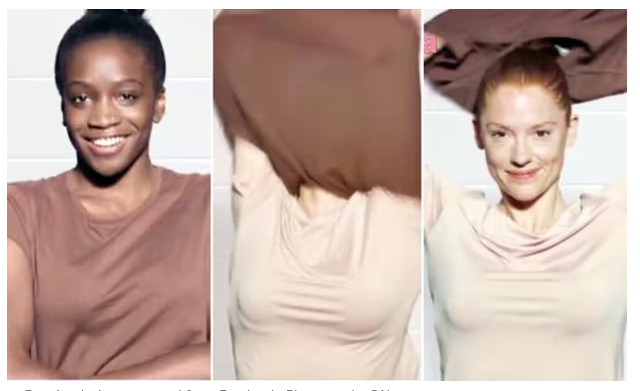
\includegraphics[scale=0.4]{Dove} \cite{Dove} This provoked an outcry, with women left wondering how a big company like Dove could make an advert that was so tone deaf. Dover had to remove the advert from Facebook and apologise. \\
        \hline
    \end{tabular}
\end{table}


The following are my own investigations

\begin{table}[htbp]
    \centering
    \begin{tabular}{|p{0.3\textwidth}|p{0.6\textwidth}|}
       \hline
       \multicolumn{1}{c}{\bfseries Company Name} & \multicolumn{1}{c}{\bfseries What was positive about it?}  \\
       \hline
	Cashmere 19 Crimes & While it can be tempting for some products to stick with a tried and tested digital advertising campaign, there is little room for new products to stand out in a very crowded arena. This is why when Cashmere launched their wine 19 Crimes they went with a broad specturm approach of using “social, broadcast, AR experiential, OOH (Out of Home) advertising , radio, audio streaming, and influencer marketing” \cite{19Crimes}. This was a huge gamble on their part as it is more expensive to use all these channels, but as cen be seen in their label where they show Snoop Dogg, they are targeting a slightly younger audience and this was seen to be the way to reach them. It remains to be seen if it did reach them but it caused enough interest that they were put in to the general consciousness.  \\
        \hline
	Dunkin\' & If a brand wants to connect with Gen Z and possibly millenials, then one way to go about that is to try to engage with influencers on TikTok. As we have seen before if this is not done by a social manager who is aware of how to engage with social media then this can spectaularly backfire. The converse of this is when it\'s done right then it can take off in a way that no other channel can, and that is what Dunkin\' did when they worked with the influencer Charli D'amelio. \cite{Dunkin} Dunkin\' time to build up a long lasting partnership with Carli D\'amelio and from this they were able to get their products shown to a younger audience. The best thing was that Dunkins\/' were able to see a material difference in their sales, they had a 57\% increase in downloads of their app and a 45\% increase in sales of cold brews. \\
        \hline
    \end{tabular}

\end{table}

\begin{table}[htbp]
    \centering
    \begin{tabular}{|p{0.3\textwidth}|p{0.6\textwidth}|}
       \hline
       \multicolumn{1}{c}{\bfseries Company Name} & \multicolumn{1}{c}{\bfseries What was negative about it?}  \\
        \hline
	Burger King & On International Women\'s day 2021, Burger King decided to promote the fact that they had a cooking scholarship for female employees. In what they thought was a humorous twist they put out a tweet reading \'Women belong in the kitchen.\' The backlash was almost immediate from many people on social media who just saw it as a sexist joke. Like most social media mistakes, the cost to the company was not published, but this is not going to have helped thier profits. The takeaway from this is that any social media campaign should at the very least be reviewed by an active social media user. \cite{BK} 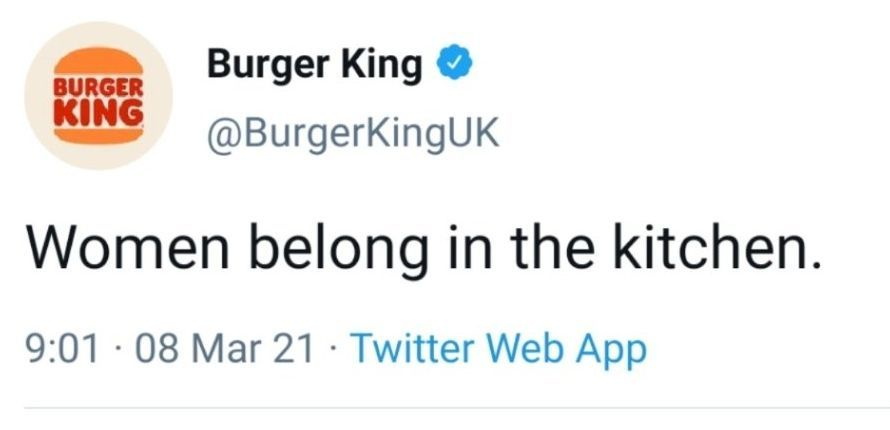
\includegraphics[scale=0.3]{BK} \\
        \hline
	Ford & Like other failures we have cataloged, what should have obviously been an area to be careful in is one where a giant coropration should have been able to identify a bad campagin. In 2017 Ford put out an advert that featured three women being bound, gagged and shoved in to the boot of a Ford hatchback. Bearing in mind this was the in the same year of \#MeToo and Harvey Weinstein, the advert blew up, in a very bad way. \cite{Ford} \\
        \hline
    \end{tabular}
\end{table}
\FloatBarrier

\section{Conclusion/Summary}


Considering that digital marketing can be a very cheap and impactly tool, it is easy to see why brands want and likely need to use it. The upside of a sucessful and thoughtout campaign can not only have an instant imapact but with hashtag and social interaction, the uptick in brand and product awareness can continue organically long after the campaign has finished. The flip side to this powerful tool is that if it is not used without consideration then the campaign can have a huge and long lasting negative impact on the brand. 
The largest takeaway from this is that most of the failures could have been avoided, in hindsight it seems almost amazing that no one noticed there were major issues with them. As digital marketing continues to mature, brands should quickly learn what is acceptable and what is not.


\bibliography{bibliography}
\end{document}

         
